\section*{Цель работы}

\begin{enumerate}
    \item Получение передаточной характеристики и семейства
    выходных характеристик полевого транзистора;
    \item Расчёт схемы автоматического смещения полевого
    транзистора;
    \item Исследование усилительного каскада по схеме с общим
    истоком.
\end{enumerate}



\section*{Исходные данные}

Все исследования, проводимые в лабораторной работе, выполняются с 
полевым транзистором HAT2164H согласно 16 варианту.
Технические характеристики транзистора:
\begin{itemize}
    \item Ток стока $I_{C}=60\ A$;
    \item Напряжение сток-исток $U_\text{\text{СИ}}=30\ \text{В}$;
    \item Пороговое напряжение затвора $U_\text{пор}=0.8\dots2.3\ \text{В}$;
    \item Рассеиваемая мощность $P=30\ \text{Вт}$.
\end{itemize}


\section*{Снятие передаточной ВАХ полевого транзистора}

Для снятия передаточной ВАХ полевого транзистора в программной среде LTspice 
соберем схему как на рисунке \ref{fig:схема_перед_вах}, после симуляции
получим график зависимости $I_C=f(U_\text{ЗИ})$ (см. Рис. \ref{fig:перед_вах}) при постоянном напряжении 
источника питания равном 10 В.


\begin{figure}[H]
    \centering
    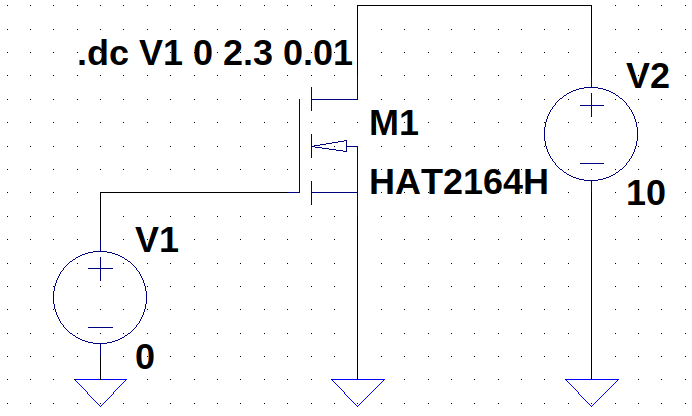
\includegraphics[width=\linewidth]{figs/task_1_scheme.png}
    \caption{Схема для снятия ВАХ полевого транзистора}
    \label{fig:схема_перед_вах}
\end{figure}

\begin{figure}[H]
    \centering
    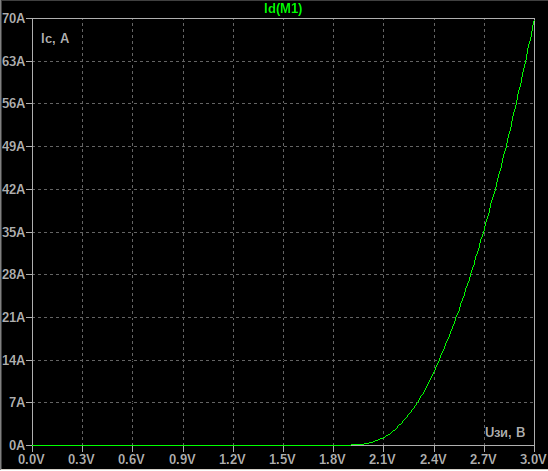
\includegraphics[width=0.8\linewidth]{figs/task_1_перед_хар.png}
    \caption{Передаточная ВАХ полевого транзистора}
    \label{fig:перед_вах}
\end{figure}



\section*{Снятие выходных ВАХ полевого транзистора}

Для получения выходной ВАХ воспользуемся той же схемой как на рисунке \ref{fig:схема_перед_вах},
зависимость $I_C=f(U_\text{СИ})$ при напряжении затвор-исток от 3 до 10 В можно
увидеть на рисунке \ref{fig:выход_вах}.

Крутизна определяется как отношение приращения тока стока $\Delta I_C=36.3\ A$ к изменению 
входного напряжения $\Delta U_\text{ЗИ}=421.6\ \text{мВ}$ при постоянном $U_\text{СИ}$
(см. Рис. \ref{fig:коэффициент_крутизны}):
\begin{equation*}
    S=\frac{\Delta I_C}{\Delta U_\text{ЗИ}}=86.2\ \frac{A}{B}.
\end{equation*}

Выходная проводимость представляет собой
дифференциальную проводимость канала транзистора и
определяется как отношение приращения тока стока $\Delta I_C=24.2\ A$ к
изменению выходного напряжения $\Delta U_\text{СИ}=12.0\ B$ при постоянном $U_\text{ЗИ}$
(см. Рис. \ref{fig:коэффициент_выходной_проводимости}):
\begin{equation*}
    G=\frac{\Delta I_C}{\Delta U_\text{СИ}}=2.0\ \frac{A}{B}.
\end{equation*}

Внутреннее (или выходное) сопротивление полевого
транзистора
\begin{equation*}
    R_i=\frac{\Delta U_\text{СИ}}{\Delta I_C}=0.5\ \text{Ом}.
\end{equation*}


\begin{figure}[H]
    \centering
    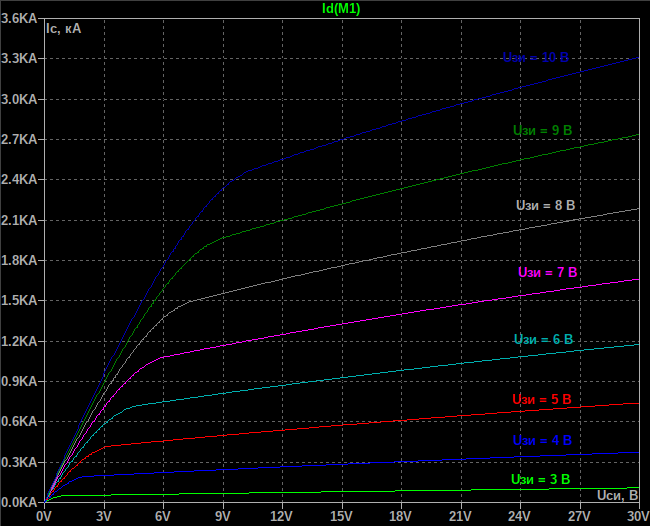
\includegraphics[width=0.8\linewidth]{figs/task_2_выход_вах.png}
    \caption{Выходная ВАХ полевого транзистора}
    \label{fig:выход_вах}
\end{figure}

\begin{figure}[H]
    \centering
    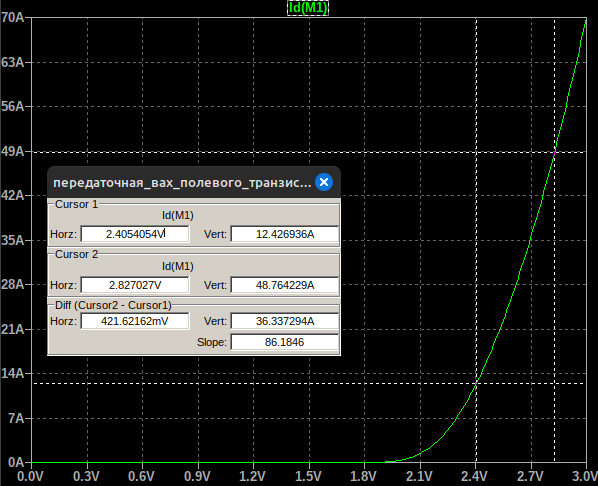
\includegraphics[width=0.8\linewidth]{figs/получение_S.png}
    \caption{Получение коэффициента крутизны}
    \label{fig:коэффициент_крутизны}
\end{figure}

\begin{figure}[H]
    \centering
    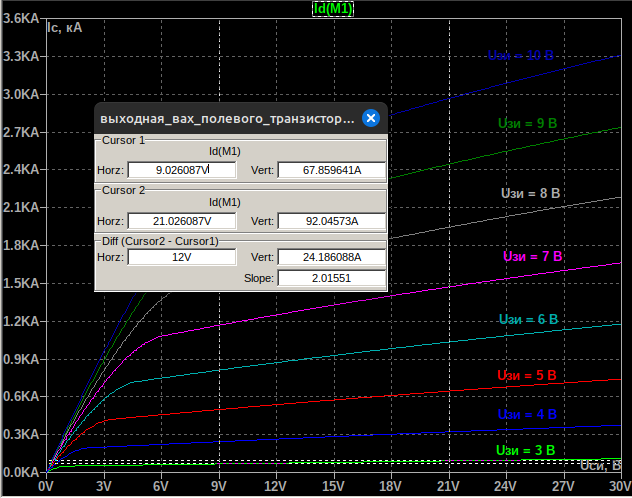
\includegraphics[width=0.8\linewidth]{figs/получение_G.png}
    \caption{Получение коэффициента выходной проводимости}
    \label{fig:коэффициент_выходной_проводимости}
\end{figure}



\section*{Задание рабочей точки усилительного каскада с общим
истоком}

На выходной ВАХ построим линию максимальной мощности (см. Рис. \ref{fig:рабочая_точка}),
выберем значение напряжения источника питания $E_\text{К}=15\ B$.
Величина сопротивления $R_C$ оказывает влияние на частотные
свойства каскада. С точки зрения расширения частотного
диапазона рекомендуется значение $R_C$ уменьшить. Нам известно 
внутреннее сопротивление транзистора, тогда значение сопротивления можно выбрать в
соответствии с соотношением $R_C=(0.05\dots 0.15)R_i$, пусть $R_C=0.1\cdot R_i=0.05\ \text{Ом}$. 

На выходной ВАХ построим нагрузочную линию. Для построения
линии рассматриваются два режима --- режим холостого
хода и короткого замыкания, соответственно находятся две
точки, через которые проходит нагрузочная линия. Обычно
выбирают величину падения напряжения на $R_\text{И}$ порядка $(0.1\dots 0.3)E_K$,
тогда пусть $R_\text{И}=0.16\cdot E_K=2.5\ \text{Ом}$. Итоговую нагрузочную линию
можно увидеть на рисунке \ref{fig:рабочая_точка} ввиде красной линии. 
Получаем точку (см. Рис. \ref{fig:рабочая_точка}):
\begin{equation*}
    U_{\text{СИ}_0}=7.3\ \text{В},\quad I_{\text{С}_0}=3.2\ A,\quad U_{\text{ЗИ}_0}=2.2\ B.
\end{equation*}

Расчет значений сопротивлений резисторов делителя. Можно задать значение
сопротивления $R_1=1\dots 2\ \text{МОм}$, пусть $R_1=1\ \text{МОм}$. 
\begin{equation*}
    R_2=\frac{E_KR_2}{U_{\text{И}_0}+U_{\text{ЗИ}_0}}-R_1=\frac{15\cdot 1e6}{8+2.2}-1e6\approx0.46\ \text{МОм}.
\end{equation*}

\begin{figure}[H]
    \centering
    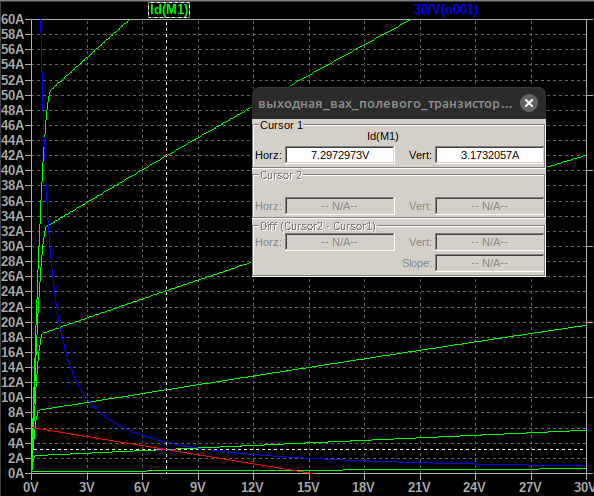
\includegraphics[width=0.8\linewidth]{figs/рабочая точка.png}
    \caption{Рабочая точка усилительного каскада с общим истоком}
    \label{fig:рабочая_точка}
\end{figure}



\section*{Заключение}



